\chapter{\Des}
  \section{Beskrivelse/teori}\label{sec:des-teori}
    \inline{Beskrivelse af tidsmodellen, teorien omkring den og hvor/hvad den 
    benyttes til. Teori: henvisning til litteratur, bl.a.  matematik/beviser 
    for modellen}
   
\subsection{Barrierer}\label{sec:barrierer}
I \des findes der i modsætningen til Parallel \des \fixme{referencer} en global 
tid og alle processerne skal derfor have en fælles tid der tæller op samtidigt.  
En global viden som tid kræver synkronisering af alle processerne\fxnote{ref}, 
og til denne koordinering og synkronisering af flere processer er den mest 
brugte metode at introducere en barriere.

Barrierer blev først introduceret i MPI\fxnote{ref}, hvor den bruges til at 
sikre at alle tråde venter i barrieren før de kan fortsætte. 

I \pycsp kan man udnytte at begge kanalender skal være klar, før der kan 
kommunikeres og at en process der er indgår i en kommunikation vil vente indtil 
den anden ende er klar før den fortsætter. Ved hjælp af kanaler kan man derfor 
lave en simpel barriere trivielt ved brug af kommunkation over kanaler. En 
implementation af en barriere som en selvstændig process kan eksempelvis 
implementeres som i \cref{barrier-imp}.

\begin{lstlisting}[float, label=barrier-imp,caption=En barriere i \pycsp]
@process
def Barrier(nprocesses, signalIN, signalOUT):
	while True:
		for i in range (nprocesses):
			signalIN()
		for i in range (nprocesses):
			signalOUT(0)
\end{lstlisting}

Denne implementation af en barriere kræver, i modsætning til de fleste andre implementationer af barrierer\cites{mpi-barrier, crew}, to kald. Det første sender en variabel til barriereprocessen, mens,
det andet kald modtager en dummyværdi fra barriereprocessen. Det kræver derved 
to kanaler at implementere barrieren. På den ene kanal er barrieren den eneste 
der læser værdierne; en besked sendt på denne kanal vil derfor altid modtages 
af barrieren. På den anden kanal er barrieren den eneste der skriver, og en 
modtaget besked må derfor komme fra barrieren.

Vi kan overbevise os om korrektheden af barrieren, da alle processerne først 
går ind i barrieren ved at sende en værdi til barrieren. Hvis barrieren ikke er 
klar, sikrer CSP at processerne venter indtil barrieren er klar til at modtage 
værdierne. Først når barrieren har modtaget en værdi fra alle processerne, 
begynder barrieren at sende sin værdi, og det er først når en proces modtager 
denne værdi fra barrieren at den må fortsætte. Når en proces modtager værdien 
fra barrieren fortsætter den og man kan risikere at den ønsker at gå ind i 
barrieren inden denne har sendt sin værdi til alle processer. Den første proces 
vil da gå i stå mens den venter på at sende sin værdi til barrieren, det skyldes at i CSP skal begge processer  være klar til at kommunikere før selve kommunikationen kan foregå, og det er denne egenskab ved kanaltransmission der  forhindrer processen i at komme foran. Først når barrieren har sendt sin værdi til alle 
processer kan den modtage værdien fra processer, og denne kan fortsætte. \fxnote{S: bedre?}

En ulempe ved denne simple barriere er at antallet af processer skal være 
konstant gennem hele kørslen.
Dette er f.eks. et problem i bankeksemplet (\cref{bank-eksempel}), hvor 
generatorfunktionen kan slutte lige efter at have genereret den sidste kunde.  
Her må den fortsætte med blot at kalde barrieren, indtil servicedisken har 
processeret alle kunderne, før hele programmet kan afslutte. Alternativt må 
barriereprocessen ændres, så den dynamisk kan ændre på hvor mange processer der 
skal synkroniseres. \inline{skal vi fortælle hvordan der kan gøres i \pycsp}

Barrierer er en meget effektiv metode til at synkronisere processer der kører parallelt, og er brugt flitigt i MPI. I \csp er der dog en konflikt i brugen af barrierer da hver proces fungerer i isolation, og den eneste interaktion der skal være mellem processerne er når der kommunikeres via kanalerne. Introduktionen af barrierer og kald til disse virker derfor kunstig i \csp. \tcite{crew} beskriver brugen af barrierer som:
\begin{otherlanguage}{english}
\begin{quote}
[\ldots] where the barriers may be used to maintain global and/or localised models of time and to synchronise safe access to shared data [\ldots]
\end{quote}
\end{otherlanguage}
Barrierens berettigelse er derfor for at kunne introducere tid, samt for at kunne bruge delt data. I \csp bør der ikke være delt data mellem processerne, men derimod kun  lokalt data. Hvis der er data er delt pga. arkitekturen \csp er implementeret på, bør dette abstraheres væk men udnyttes internt i kanalerne. At introducere hjælpemidler for styre delt data, er derfor at tilskynde til en forkert brug af \csp. Tiden er den anden begrundelse for at benytte barrierer. Men med brugen af barrierer til at modellerer tid, kan man får  en primitiv model for tid, og vi vil i vores speciale vise ved at inkluderer tid i stedet får man et stærkere værktøj der ud over en masse andet også kan erstatte brugen af barrierer.\inline{det sidste er helt tosset og skal hives et niveau op tekstmæssigt}

\section{Eksempel}
\fxnote[inline]{Beskrivelse af eksemplet og hvordan det er relateret til problemet/modellen. Beskrivelse af løsning uden vores tid}


\subsection{Hajer og fisk på Wator} Som et eksempel på en \des har vi valgt at 
tage  udgangspunkt i det scenarie som A. K. Dewdney
beskrev i artiklen \citetitle{wator}\cite{wator}. Artiklen beskriver den
fiktive planet Wator, der har form som en torus og er fuldstændig
dækket af vand. Verdenen er inddelt i felter \cite[20]{wator}, som kan være tomme, indeholde en
fisk eller en haj. Følgende karakteristika beskriver fisk og hajers
opførsel.

\begin{itemize}
\item[\textbf{Fisk}]
Lever af plankton, en ressource som er uendelig. Hvis der er èt ledigt 
tilstødende felt, bevæger den sig til dette felt. Hvis der er flere ledige 
felter vælges et tilfældigt. Såfremt en fisk overlever 3 tidsskridt forplanter 
den sig.
\item[\textbf{Hajer}]
Såfremt der er fisk i et eller flere tilstødende felter, vil hajen bevæge sig 
til et af disse felter og spise fisken. Hvis der er ikke er nogen fisk i et af 
disse felter flytter hajen sig til et tilfældigt valgt ledigt felt. Hvis en haj 
ikke spiser i 3 tidsskridt dør den. Overlever den i 10 tidsskridt forplanter 
den sig.
\end{itemize}

For hvert tidsskridt vil alle fisk og hajer udføre en handling ud fra
ovenstående opførsel.
Til at initiere systemet skal der defineres en størrelse af verdenen,
samt hvor mange fisk og hajer der er til stede fra start. Disse fisk og
hajer placeres tilfældigt i verdenen.
Såfremt de initielle parametre for antal fisk og hajer understøtter en 
bæredygtig bestand forventer vi at se bestanden af henholdsvis fisk og hajer 
oscillerer afhængigt af hinanden.

Vi har valgt dette eksempel, da det er enkelt og let forståeligt, men samtidig 
introducerer problemstillinger omkring synkronisering når det paralleliseres.  
Disse problemstillinger optræder fordi en opdatering af hvert felt er afhængigt 
af de omkringliggende felter, og vil derfor være afhængig af felter fra andre 
processer i grænsetilfælde. Ud over at være afhængig af information fra andre 
processer, kan en opdatering også påvirke data hos andre processer.   

\subsubsection*{Før introduktion af et tidsbegreb i CSP} For at simulere Wator 
verdenen i et CSP-system hvori tidsbegrebet ikke er introduceret, er vi nødt 
til at udføre en synkronisering af de enkelte processers arbejde. Denne 
synkronisering kan ske ved brug af barrierer, hvor alle processer udfører en 
handling og mødes i barrieren før de fortsætter.

Vi har valgt at basere vores model på \citetitle{crew}\cite{crew}\fxnote{Brian: 
Hvad er din holdning til litteraturhenvisninger.}, hvor verdenen repræsenteres 
som en delt datastruktur og adgangen til denne styres med barrierer. I vores 
model er hver proces derved ansvarlig for en del af verdenen og tilgangen til 
den delte datastruktur sker ud fra CREW-princippet (Concurrent Read, Exclusive 
Write)\cite[5]{crew}, der styres vha. barrierer.  

I en mere ren CSP-model ville man foretage en direkte udveksling af data mellem 
processerne, og undgå den delte datastruktur vi har i vores model.  Vi har 
valgt denne model frem for den mere rene CSP model, da den klarlægger brugen af 
barrierer bedre.  Det bliver meget eksplicit i koden hvornår hvilke dele 
opdateres, og hvornår processerne venter i en barriere.

Vi deler verdenen lodret, hvor hver proces styrer en verdensdel. Hver proces 
gennemgår sin verdensdel og udfører en mulig handling for hver fisk og haj, dog 
vil fisk og hajer i de sidste to kolonner i hver verdensdel ikke bliver 
opdateret på nuværende tidspunkt. Dette skyldes at der kan opstå en en race 
condition hvis disse to kolonner opdateres samtidig med de andre. Årsagen til 
dette er at både processen der er ansvarlig for kolonnerne, og processen 
umiddelbart til højre for den skal have mulighed for at flytte fisk og hajer 
ind i dette område. Hvis der i samme tidsskridt er mulighed for at flytte dem 
ud af området, vil opførslen afhænge af hvad der sker først.  Når denne 
opdatering er fuldført mødes processerne i en barriere, hvorefter hver proces 
opdaterer de to sidste kolonner. Herefter mødes processerne igen i barrieren, 
og når alle kolonner er opdateret kan der foretages en visualisering af de 
udførte opdateringer. Til slut mødes alle i en barriere igen før processerne 
kan begynde en ny iteration.

En repræsentation af opdelingen ses på \cref{fig:wator}. Her er verdenen 
opdelt mellem to processer, og de to kolonner mellem hver del opdateres i et 
separat tidsskridt.  

\begin{figure}[hbtp] \begin{center}
  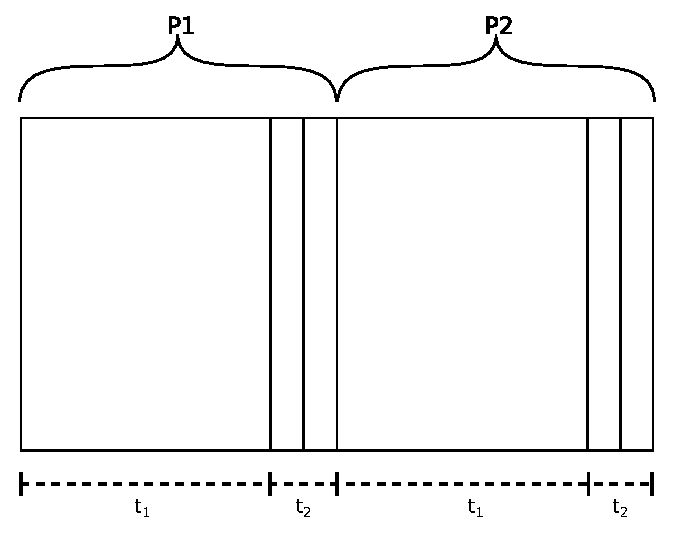
\includegraphics[scale=0.75]{images/wator}
  \caption{Opdeling af verdenen mellem to processer. Der er for hver verdensdel 
  to kolonner som opdateres i et separat tidsskridt.}
  \label{fig:wator}
  \end{center}
\end{figure}


\begin{figure}[hbtp]
\begin{minipage}{\linewidth}
\begin{lstlisting}[label=code:wator-worldpart,caption=Uddrag af processen 
  \code{worldpart} i Wator]
  @process
  def worldpart (part_id, barR, barW):
  
  ...
  
    while True:
      #Calc your world part:
      main_iteration()
      barW(1)
      barR()
      #Update the two shadowcolumns
      for i in range(world_height):
        for j in range(2):
          element_iteration(Point(right_shadow_col+j,i))
      barW(1)
      barR()
      #visualize have single access
      barW(1)
      barR()
\end{lstlisting}

\begin{lstlisting}[label=code:wator-visualize,caption=Processen 
  \emph{visualize} i Wator]
@process
 def visualize(barR,barW):
   for i in xrange(iterations):
     barW(1)
     barR()
     barW(1)
     barR()
     pygame.display.flip()
     barW(1)
     barR()
   poison(barW,barR)
\end{lstlisting}

\end{minipage}
\caption[test]{\code{barW(1)} og \code{barR()} er henholdsvis skrivning og læsning til og 
fra en barriere som defineret i \cref{sec:barrierer}.}
\end{figure}
Afviklingen af programmet sker ved at et antal \emph{worldpart}-, en 
\emph{visualize}- og en \emph{barrier}-process køres parallelt. Af 
\autoref{code:wator-worldpart} og \pageref{code:wator-visualize}\fixme{ændrer pageref til vref i final}, ses det 
overordnede design af henholdsvis \emph{worldpart}- og 
\emph{vizualize}processen.  Værd at bemærke er det store antal barrierekald i 
visualizeprocessen. Dette er til for at man kan benytte den samme barriere som 
wordpartprocessen. Alternativt kunne man have to barriereprocesser; en til 
synkronisering af \emph{worldpart} med \emph{vizualize}, samt en som 
\emph{worldpart}processerne brugte til synkroniseringen af opdatering af 
verdensdelen og de to sidste kolonner.\fixme{hvad skal emphs og hvad skal med stå med code og hvad skal fjernes.} 

\fxnote{konklusion hvordan var det at implementere og hvor stor parallelitet 
kan man opnå. }


\subsection{Kunder i en bank}\label{bank-eksempel}
Et klassisk eksempel inden for \des er at simulere  en række kunder der alle 
ankommer til en butik, hvor de skal serviceres. Dette simple problem kan 
udvides til at modellere mange forskellige problemstillinger, der berører 
hvordan flowet ændrer sig hvis man varier en eller flere parametre
i systemet. Programmeringssproget \simpy\fxnote{ref}har, som et af deres 
eksempler, en simulering af kunder i en bank. \simpy bruger dette som et 
gennemgående eksempel, hvor de løbende udvider modellen, for at vise 
forskellige egenskaber ved \simpy. For at kunne sammenligne \simpy  med vores 
implementation af logisk tid, vil vi implementere to af eksemplerne med kunder 
i en bank i \pycsp.

I det simple tilfælde af eksemplet ankommer kunderne til banken på 
tilfældige tidspunkter.  De opholder sig i banken i et tilfældigt 
tidsrum, hvorefter de igen forlader banken. I dette eksempel kan der ikke 
uddrages meget information, men det viser hvordan en simpel model er opbygget i 
hhv.  \simpy og \pycsp for at håndtere tid.\inline{bedre ental/flertal}

I det andet eksempel er modellen udvidet med en servicedisk. Her skal alle 
kunderne betjenes af en servicemedarbejder, som kun kan ekspederes en kunde ad 
gangen. Alle kunder ankommer igen til banken i tilfældig orden og stiller sig i 
kø for at blive serviceret. Dette  svare til en M/M/1\fixme{hvad  er en m/m/1 
kø} kø. Det er igen et tilfældigt tidsrum som kunden bruger på at blive 
serviceret.  Dette er stadigt en meget simpel model, men med introduktionen af 
en begrænset ressource kan man uddrage information om den tilhørende kø, f.eks. 
kan der måles hvor lang det tager for hver kunde at blive betjent af 
servicemedarbejdere, samt hvordan køen opfører sig over tid. 

\subsubsection{Før introduktion af et tidsbegreb i \pycsp}
I \simpy er kunderne en proces og det vil derfor være nærliggende ligeledes at 
modellere eksemplet i \pycsp med kunder som en proces. Dette sker i  \simpy når
generatorfunktionen laver en kunde og lader denne køre parallelt med sig selv.  
I \pycsp,\fxnote{hvorfor?- kan man lave child proces der køre i samme parallel 
kald som dets parent?} er standard metoden\fxnote{set fra kodeeksempler}, at 
modellere mere statiske processer, gerne med en generator- og 
arbejderproces, og lade arbejdet flyttes 
mellem processerne igennem kanaler. I \pycsp modellen fungerer 
generatorprocessen som i \simpy, men vi introducerer en bankproces 
som arbejder, og lader kunderne være arbejdet der flyttes mellem dem. 

Mens \simpy kalder kundeprocessen fra generatoren og lader denne stå for håndteringen af kunden 
og den tid hun befinder sig i banken, kender bankprocessen i \pycsp ikke tid som 
sådan. Bankprocessen skal derfor selv vedligeholde en liste med kunderne, der findes inden i banken og til hver 
tidskridt vide hvilke kunder der skal forlade den. 

Tiden er igen modelleret ved brug af barrierer, se afsnit \cref{sec:barrierer}. I 
stedet for at have de to kald til barrieren som den kræver, lige efter hinanden, lader 
vi bankprocessen gå ind i barrieren i starten af tidsskridtet, og så modtage 
kunder, indtil bankeprocessen modtager det andet kald fra barrieren(se 
\cref{bank-alternation-imp}). Dette er nødvendigt for at lade banken have 
mulighed for at modtage et vilkårligt antal kunder i samme tidsskridt, samt 
vide hvornår der ikke vil komme flere kunder.  Vi kan ræsonnere os frem til at 
barrieren stadig virker efter hensigten ved  simpel indsigt.
For at generatorprocessen kan komme foran med et tidsskridt og sende en kunde i et forkert tidsskridt,
skal den have fuldført begge begge kald til barrieren, mens bankprocessen ikke 
har modtaget et kald fra barrieren. Barrieren vil dog ikke modtage kald fra 
nogle, før den har  kaldt bankprocessen. Derfor må generatorprocessen vente i 
sit første kald til barrieren, indtil banken har modtaget sit kald fra 
barrieren, før den kan sende en ny kunde.
Når bankprocessen har modtaget et kald fra barrieren er den ikke længere villig 
til at modtage kunder, før i det efterfølgende tidsskridt. Vi kan bruge samme 
analogi til at ræsonnere os frem til at bankprocessen ikke kan komme et 
tidsskridt foran generatorfunktionen, og derfor virker barrieren stadigt som 
forventet. 

\begin{lstlisting}[float=hbtp,label=bank-alternation-imp,caption=Modtage en 
  kunde eller barrierekald i Bankprocessen]
while True:
		(g,msg) = Alternation([{
		barrierREADER:None,
    customerREADER:None
    }]).select()
		if g == barrierREADER:
			break
    elif g == customerREADER:
			heappush(customers,(time+msg.waittime,msg))
\end{lstlisting}


I det mere avancerede eksempel hvor kunderne skal tilgå den samme begrænsede 
ressource dannes en kø. Denne kan i \pycsp modeleres på flere måder, afhængigt 
at hvilken proces der skal have ansvaret for at vedligeholde køen. En metode er 
internt i en proces at have en liste af kunder der venter, og lade det være 
processens ansvar at håndtere denne liste som en kø. Processen med ansvaret for køen kan 
så enten være den begrænsede ressource, eller en separat proces hvis eneste 
formål er at vedligeholde køen. For nyligt\footnote{d. 22. december 2009} er 
der i \pycsp blevet introduceret ''buffered channels''\cite{pycsp-r147}, og 
disse kan også bruges som en kø. Dermed kan man modellere sin ressource uden 
hensyntagen til håndtering af køen internt eller vha. andre processer, og blot 
lade processen læse fra kanalen når den er klar. Vi har i dette eksempel valgt 
at lade køen være repræsenteret ved en ''buffered channel'', da denne  kræver 
færrest linjer kode, men den kunne lige så godt være repræsenteret som en liste 
i servicedisk processen.


\subsubsection*{Konklusion - evaluering - ?}
Ved at se på  implementationen af de to eksempler af kunder i en bank sammenholdt med implementationen i \simpy kan man se at de egner det sig godt til 
simulering, og fra eksemplet kan man se at der findes meget kode til 
vedligeholdes af de interne tidsvariabler, som \simpy ikke har behov for. Det drejer sig 
om kode der sørger for at hver proces kender tiden, samt at den er 
synkroniseret på tværs af processerne. Vi forventer derfor at koden skal kunne 
simplificeres i \pycsp med tid, så det bliver lige så simpelt at implementere som i 
\simpy. 

I \simpy findes begrebet ressource direkte i sproget, som en type og 
servicedisken er blot en instans af denne type, og ressourcen står selv for at 
håndtere køen. I \pycsp modelleres servicedisken som en separat proces, og 
bankprocessen er defor reduceret til blot at sende kunden videre til 
servicedisken og lade kanalen håndtere køen. En ulempe ved brugen af ''buffered 
channels'' som en kø er, at kanalen har en fast størrelse på sin buffer, som 
angives når kanalen oprettes. Man kan dermed risikere en deadlock ved brug af ''buffered 
channels'' sammen med barrierer. Dette opstår hvis ikke processen i samme 
tidsskridt kan foretage transmissionen og kalde barrieren.
Dette kan løses med en alternation og skip guard\inline{find en standard som vi 
bruger til at referere til kode-elementer med, fx emph, tt eller andet}, men så 
skal bankprocessen håndtere fejlede forsendelser og må nødvendigvis introducere en 
sekundær kø hvilket gør at introduktionen af en ''buffered channel'' er 
irrelevant. For undgå dette har vi i vores tilfælde valgt blot at 
angive en maksimal størrelse på bufferen som er større end det totale antal 
kunder banken modtager.

  \section{Design og implementation}
    \fxnote[inline]{Beskrivelse af design med udgangspunkt i eksemplet}
    Formålet med introduktionen er to ting. Dels ønsker vi at introducere diskret tid som et alternativ til barrierer. Dels ønsker vi med diskret tid at åbne for mulighederne for at kunne foretage simuleringer, hvor man bruger \csp som model for systemet. Med disse ændringer er håbet at vi opnår en model der ligger tætter på intentionen bag \csp og så man kan udfase brugen af barrierer, samt med den underliggende parallelitet i \csp kan udnyttes til at øge hastigheden af de simulere modeller, hvis de er begrænset af beregningskapaciteten.
    
Der findes et åbenlyst problem med introduktionen a \des i \csp, som vi kort berørte i \cref{sec:barrierer}. Dette er at \csp er lavet med henblik på at  ligestillede processer der arbejder samtidigt, og uafhængigt af hinanden, mens \des  ikke er parallelt, men skedulere sine begivenheder linært efter hvornår de sker og så kronologisk \fxnote{Dette skal vidst i teori}løber begivenhederne igennem, til der enten ikke er flere begivenheder eller tiden når et vidst punkt. Alternativet til  \des  er \pdes hvor processerne kan have at tiden løbe uafhængigt af hinanden. Dette introducere muligheden for størrer parallelitet, men samtidigt risikere de processerne ved kommunikation at modtage beskeder fra fortiden, som der skal tages hånd om, f.eks. ved at rulle tiden tilbage. Det har der vidst sig at omkostningerne ved at lade tiden kører parallelt er omkostningerne størrer end ved at holde tiden synkront på tværs af processerne.
    
I \pycsp findes der tre versioner der implementerer \csp: \emph{Process, threads, greenlets}\cite{Friborg2009}. Muligheden for at introducere \des, i de forskellige versioner afhænger af hvordan processerne styres, og dermed hvordan \des kan  implementeres i de forskellige versioner. I process og threads versionen af \pycsp styres processerne af operativsystemet uafhængig af hinanden \inline{ref?}. Når \pycsp afgiver kontrollen med processerne kører de parallel, men samtidigt har \pycsp ikke mulighed for fra  et central område at diktere tiden i de forskellige processer. I greenlets køres processerne på bruger-nivau som en del af Python. Processerne har ikke mulighed for at køre parallelt, og processerne fortsætter med deres kørsel indtil de frivilligt afgive kontrol. Til gengæld findes der central scheduler der står for koordinering af de forskellige processer. 
    \section{Repræcentation af tid}

I PyCSP foregår kommunikation kun når begge kanalender er klar dvs.
når der findes både en kanalende der vil skrive og en kanalende der vil læse. 
Hvis kun en af kanalenderne er klar, vil den vente indtil
der findes minumum en kanalende af hver type, der er klar. I alternation 
findes muligheden for at tilknytte en timeout til en guard. Dette
giver muligheden for at en process, kun er villig til at vente på at kanalen 
bliver klar inden for en given tidsperiode. 
\begin{lstlisting}[label=Timeout,
  caption=Timeout i Alternation (fra dokumentationen til PyCSP)]
  Alternation([{Timeout(seconds=0.5):None},
               {Cin:None}]).select()
\end{lstlisting} 

I denne alternation er processen villig til at læse fra Cin i 0.5 sekunder. 
Ellers accepteres timeoutguarden og processen er ikke længere villig til at 
læse fra Cin.

Med et simuleringsmiljø er det ikke nok udelukkende kan kunne specifiere en 
timeout på kanalen, det er også nødvændigt at man kan specificere at en proces 
er villig til at kommunikere fra et tidspunkt, samt at den kanalen kun er 
villig til at kommunikere på nuværende tidpunkt, men ikke ud i fremtiden. 

At ville kommunikere fra et given tidspunkt i fremtiden,  svare til at vente 
uden at lave noget indtil det givne tidspunkt for så at forsøge at kommunikere 
fra tidpunktet indtil det kommunktationen lykedes. Dette kan dermed laves helt 
uden en alternation, men ved blot med de to funktioner Wait(time), Cin(). 

At ville være villig til at kommuikere til et given tidspunkt, medfører en ny 
problemstilling, da det introducere muligheden for deadlocks og 
nondeterminisme\fxnote{Er det korrekt?}, for det er ikke defineret hvad tiden 
er hvis det ikke lykkedes at kommunikere i det givne tidsskridt. Der findes to 
muligheder, enten skal scheduleren signalere at der ikke findes mere arbejde 
til dette tidsskridt, og lade processerne fortsætte i samme tidsskridt. 
Alternativt skal tiden tælles op til næste event, hvorefter processerne 
signaleres med at kommunkationen ikke lykkedes. Hvis processerne signalleres 
i samme tidsskridt kan man vælge enten at signallere hver proces en af gangen 
eller samtidigt at signallerer alle processerne. ingen af mulig

processen fortsætte  tildet under antagelsen af problemer.




når tiden er  tidspunkt
til for et findes der allerede \fxnote[inline]{vi skal kunne angive
at vi ønsker at kommunikere men KUN i det tidsskridt vi er i, og at
hvis dette ikke kan lade sig gøre skal vi breake noget alla at have en
timeout på 0} 
 
    \subsection{Hvordan skal events gemmes}
    
  \section{Evaluering}
    \fxnote[inline]{Evaluering af hvordan eksemplet løses efter den valgte 
    implementation benyttes. Inkluderer test+performance}
  \section{Freamtidigt arbejde}
  \section{Opsummering}
